\section{Resultados}

\subsection{Assinatura}

    Podemos ver pela \cref{fig:assinatura} que assinatura digitais, normalmente com menos de caracteres, são imperceptíveis na imagem como um todo. No plano de bit específico, a diferença também não é visível ao olho humano.

    O resultado na \cref{fig:assinatura:imagem} contém o texto ``Realizzato da Leonardo da Vinci™'', representado em UTF-8 por 35 bytes. Juntamente com o cabeçalho de 8 bytes, a assinatura ocupa 344 bits do plano menos significativo. Isso não chega a metade da primeira linha ($256 \times 3$ bits de capacidade).

    A imagem pode ser produzida por:

    \begin{minted}{bash}
        $ echo Realizzato da Leonardo da Vinci™ | python3 codificar.py imagens/monalisa.png -o saida.png
    \end{minted}

    E verficada com:

    \begin{minted}{bash}
        $ python3 decodificar.py saida.png
        Realizzato da Leonardo da Vinci™
        $ # OU
        $ python3 decodificar.py saida.png | diff -qs - <(echo Realizzato da Leonardo da Vinci™)
        Files - and /proc/self/fd/12 are identical
    \end{minted}

    \begin{figure}[H]
    \centering
    \begin{subfigure}{0.5\textwidth}
        \centering
        \includegraphics[width=0.85\textwidth]{mona_assin/imagem.png}
        \caption{Imagem com mensagem oculta.}
        \label{fig:assinatura:imagem}
    \end{subfigure}%
    \begin{subfigure}{0.5\textwidth}
        \centering
        \includegraphics[width=0.85\textwidth]{mona_assin/plano0.png}
        \caption{Plano 0.}
        \label{fig:assinatura:plano}
    \end{subfigure}\\[8pt]
    \begin{subfigure}{0.33\textwidth}
        \centering
        \includegraphics[width=0.85\textwidth]{mona_assin/pl0chb.png}
        \caption{Plano 0, canal azul.}
        \label{fig:assinatura:blue}
    \end{subfigure}%
    \begin{subfigure}{0.33\textwidth}
        \centering
        \includegraphics[width=0.85\textwidth]{mona_assin/pl0chg.png}
        \caption{Plano 0, canal verde.}
        \label{fig:assinatura:green}
    \end{subfigure}%
    \begin{subfigure}{0.33\textwidth}
        \centering
        \includegraphics[width=0.85\textwidth]{mona_assin/pl0chr.png}
        \caption{Plano 0, canal vermelho.}
        \label{fig:assinatura:red}
    \end{subfigure}%

    \caption{\texttt{monalisa.png} com uma assinatura de 35 bytes.}
    \label{fig:assinatura}
\end{figure}

\subsection{Texto Pequeno}

    \begin{figure}[H]
    \centering
    \begin{subfigure}{0.4\textwidth}
        \centering
        \includegraphics[width=0.85\textwidth]{pep_peq/imagem.png}
        \caption{Imagem com mensagem oculta.}
        \label{fig:pequeno:imagem}
    \end{subfigure}%
    \begin{subfigure}{0.4\textwidth}
        \centering
        \includegraphics[width=0.85\textwidth]{pep_peq/plano0.png}
        \caption{Plano 0.}
        \label{fig:pequeno:plano}
    \end{subfigure}\\[8pt]
    \begin{subfigure}{0.28\textwidth}
        \centering
        \includegraphics[width=0.85\textwidth]{pep_peq/pl0chb.png}
        \caption{Plano 0, canal azul.}
        \label{fig:pequeno:blue}
    \end{subfigure}%
    \begin{subfigure}{0.28\textwidth}
        \centering
        \includegraphics[width=0.85\textwidth]{pep_peq/pl0chg.png}
        \caption{Plano 0, canal verde.}
        \label{fig:pequeno:green}
    \end{subfigure}%
    \begin{subfigure}{0.28\textwidth}
        \centering
        \includegraphics[width=0.85\textwidth]{pep_peq/pl0chr.png}
        \caption{Plano 0, canal vermelho.}
        \label{fig:pequeno:red}
    \end{subfigure}%

    \caption{\texttt{peppers.png} com o \texttt{enunciado.md}.}
    \label{fig:pequeno}
\end{figure}

%% TODO %%
%
% Geral
% x Assinatura [mon]
% x Texto Pequeno [mon][wat]
% - Texto Grande [bab|pep]
% - Binario (Imagem / Zip) [bab|pep]
%
% Permutado
% - Texto Pequeno [mon] -- Tamanho + Chave
% - Texto Grande [bab|pep]
% - ?: Binário
%
% Plano de bit
% - 0, 1, 2
% - ?: 3, 5, 7
